\documentclass{tufte-handout}

%\geometry{showframe}% for debugging purposes -- displays the margins
\usepackage{amsmath}
\usepackage{amssymb}
\usepackage{siunitx}
%\usepackage{mparhack}
% Set up the images/graphics package
\usepackage{graphicx}
\usepackage{float}
\usepackage{booktabs}
\setkeys{Gin}{width=\linewidth,totalheight=\textheight,keepaspectratio}
\graphicspath{{graphics/}}
\title{Eduqas Physics Practicals for AS Physics\thanks{Remember that the practicals may not be exactly as below}}
\author[]{Exeter Mathematics School}
\date{2 Jan 2017}  % if the \date{} command is left out, the current date will be used

% The following package makes prettier tables.  We're all about the bling!
\usepackage{booktabs}
\setcounter{tocdepth}{1}

% The units package provides nice, non-stacked fractions and better spacing
% for units.
\usepackage{units}
\usepackage{siunitx}
% The fancyvrb package lets us customize the formatting of verbatim
% environments.  We use a slightly smaller font.
\usepackage{fancyvrb}
\fvset{fontsize=\normalsize}

% Small sections of multiple columns
\usepackage{multicol}
\newcounter{question}
% Provides  
% These commands are used to pretty-print LaTeX commands
\newcommand{\doccmd}[1]{\texttt{\textbackslash#1}}% command name -- adds backslash automatically
\newcommand{\docopt}[1]{\ensuremath{\langle}\textrm{\textit{#1}}\ensuremath{\rangle}}% optional command argument
\newcommand{\docarg}[1]{\textrm{\textit{#1}}}% (required) command argument
\newenvironment{docspec}{\begin{quote}\noindent}{\end{quote}}% command specification environment
\newcommand{\docenv}[1]{\textsf{#1}}% environment name
\newcommand{\docpkg}[1]{\texttt{#1}}% package name
\newcommand{\doccls}[1]{\texttt{#1}}% document class name
\newcommand{\docclsopt}[1]{\texttt{#1}}% document class option name


\newcommand{\parnum}{\bfseries\arabic{parcount}}

\newcounter{parcount}
\newcommand\p{%
    \stepcounter{parcount}%
    \leavevmode\marginpar[\hfill\parnum]{\parnum}%
}
\begin{document}

\maketitle% this prints the handout title, author, and date

\begin{abstract}
\noindent This document covers the core practicals from the Eduqas AS physics specification. The practicals may be conducted with different methods, the important thing is to learn the principles, aims, and techniques, rather than the exact methods.
\end{abstract}

%\printclassoptions
\tableofcontents
%\listoffigures
%%%%%%%%%%%
\newpage
\section{Measurement of the density of solids}
\subsection{Theory}
The density of regularly shaped solids can be determined by measuring their mass, m, and
calculating their volume, $V$. The density, $\rho$, can then be found using:
 \[ \rho = \frac{m}{V}\]


\subsection{Apparatus}
\begin{itemize}

\item Various regularly shaped solids both rectangular and circular,
\item 30 cm ruler (resolution \SI{\pm 0.1}{cm})
\item Vernier calipers / micrometer (resolution \SI{\pm 0.01}{mm})
\item Balance (resolution \SI{\pm 0.1}{g})
\end{itemize}
\subsection{Experimental Method}
Determine the mass of the object using the balance. 
The volume of a rectangle can be found by measuring the length, $l$, width, $w$, and height, $h$. Calculate the volume, $V$ using:
\[V = l  w  h\]
The volume of a sphere is found by measuring the diameter to find the radius, r, and then calculate the volume using: \[ V= \frac{4}{3} \pi r^{3}\] \sidenote{Irregular shapes are harder to measure, so we use the Archimedian principle and a water displacement can to measure the volume. If faced with a buoyant object you can weigh it down with another object, so long as you subtract the volume of that weight from the total volume of water displaced.}
\begin{marginfigure}
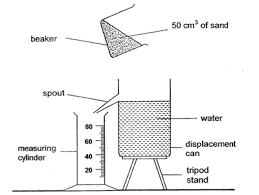
\includegraphics{eurekacan.png}
\caption{Displacement can in use.}
\end{marginfigure} 
In both cases calculate the density using: $ \rho = m/V$.
%%%%%%%%%%%%%%%%%%%%%%%%%%%%%%%%%%%%%%%%%%%%%%%%%%%%%%%%%
%\newpage
\section{Determination of unknown masses by using the principle of moments}
\subsection{Theory:}  
Apply the principle of moments to a metre rule to first determine its mass and then determine the mass of an unknown object.   
\subsection{Apparatus:} 
\begin{itemize}
\item Meter rule Clamp and stand 
\item Nail 
\item 200 g mass and hanger 
\item 150 g mass (covered in tape and labelled as W) and hanger 
\item Loops of thread           
\end{itemize}
\subsection {Experimental Method:}  
Loop a 200 g (1.96 N) mass over the metre rule and adjust it until the ruler is horizontal. Note down the distance, $x$, of the mass from the pivot. The mass (or weight) of the metre rule can now be calculated using the principle of moments:  
\begin{figure}
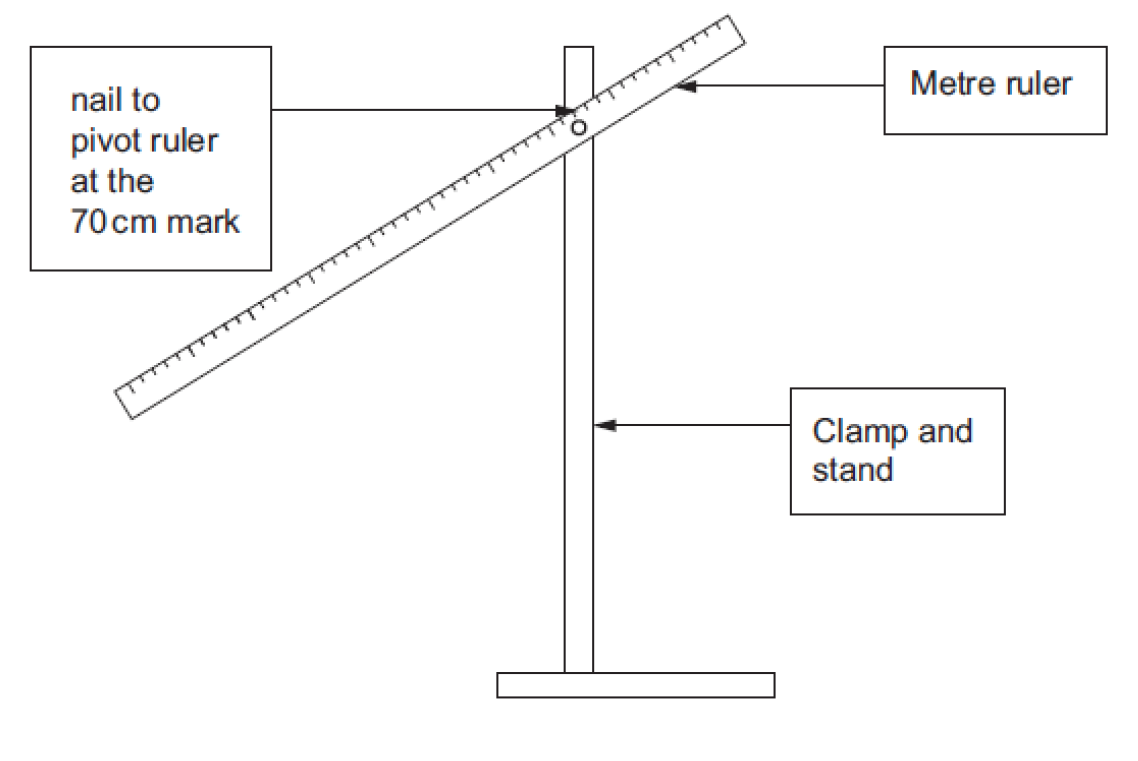
\includegraphics[width=\textwidth]{moments.PNG}
\caption{Experimental set-up for the measurement of an unknown mass by moments. It would be possible to use a knife-edge fulcrum (pivot) instead}
\end{figure}
\[0.20 \times \text{metre rule weight} = 1.96 \times x\] Now remove the 200 g mass and replace it with the unknown weight, W, and again adjust the position of the weight until the ruler balances. Measure the distance, d, of the unknown weight from the pivot. The unknown weight can again be calculated by applying the principle of moments: 

\[0.20 \times \text{metre rule weight} = d \times \text{unknown weight} \]

The unknown weight can be converted into a mass (in kilograms) by dividing by 9.81. This can then be checked using a top pan balance.\sidenote{better to use the term ``Top-pan balance'' than ``scales''} 
%%%%%%%%%%%%%%%%%%%%%%%%%%%%%%%%%%%%%%%%%%%%%%%%%%%%%%%%%%%%%%%%%%%%%
%\newpage
\section{Measurement of g by freefall}
\subsection{Theory:} 

An equation of motion can be used to calculate the acceleration due to gravity, g.\sidenote{There are two common alternative methods to the one below. \begin{enumerate}
\item Manual timing - This method has a lot of inherent errors, and gives poor results. One of the biggest sources is the approx \SI{0.3}{s} it takes to start and stop a manual timer. The next most significant are usually parallax and air resistance.
\item Using lightgates - Lightgates are very accurate, and a viable alternative for high precision results
\end{enumerate} All of these methods rely on the same basic equations of motion} 
\begin {align} 
s &= ut + \frac{1}{2}mv^{2} \\
    Where:  u &= \text{initial velocity} = 0,   \\    s &= \text{height, h and}  \\     a &= \text{acceleration due to gravity, } g \\ 
    \text{This gives } h &= \frac{1}{2}gt^{2}\\
    \end{align}
If a graph of height, $h$, (y-axis) is plotted against time squared, $t^{2}$, (x-axis) the gradient will equal g/2, or $g = 2\times \text{gradient}$.  
\subsection{Apparatus:}  

\begin{figure}
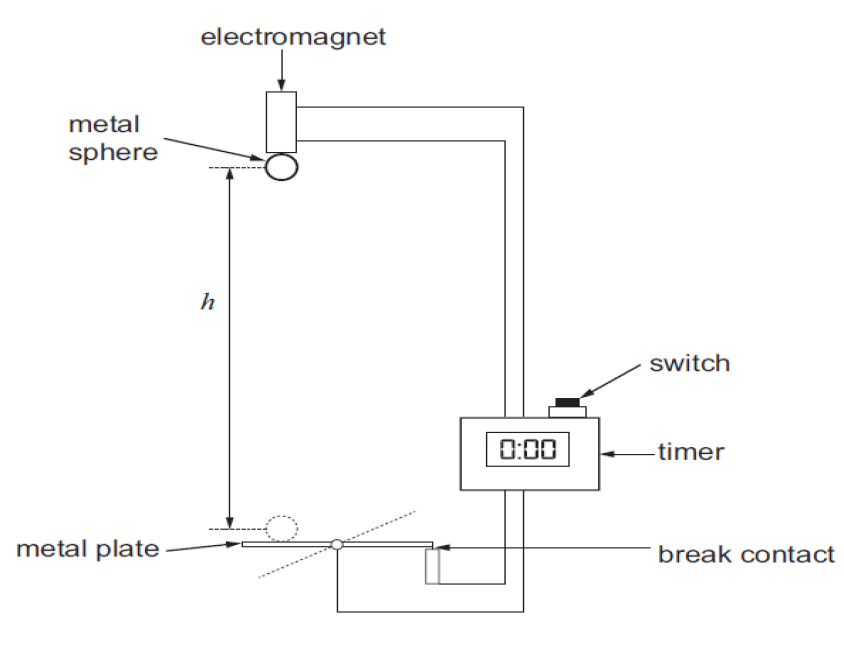
\includegraphics[width=\textwidth]{gbyfree.PNG}
\caption{``g'' by freefall}
\end{figure}

\subsection{Experimental Method:}  
When the switch is pressed it disconnects the electromagnet releasing the metal sphere\sidenote{One of the problems with this method is that the de-magnetisation of the coil is not instant. To minimise the time delay we use a soft-iron ball}. At the same instant the timer starts. When the sphere hits the magnetic switch it breaks the circuit stopping the timer, thus recording the time it takes for the sphere to fall through a height, $h$. The time taken for the ball bearing to fall through a range of different heights needs to be measured. Plot a graph of height, $h$, (y-axis) against time squared, $t^{2}$, (x-axis) and calculate the value of $g$ using:  $g = 2/gradient$. 

%%%%%%%%%%%
%\newpage
\section{Investigation of Newton's 2nd law}

\subsection{Theory:}  
The gravitational force of the slotted masses attached via the pulley causes the entire mass of the system to accelerate. That is the mass of the rider, M, and the total mass of the slotted masses, m. Newton’s second law, therefore, can be written as:  
\[mg=(M+m)a\]
and so the acceleration of the system is:  
\[a=\frac{mg}{(M+m)}\]  
We can use this to test Newton's second law. If the total mass of the system ($M + m$) remains constant\sidenote{This is \emph{really} important and is the reason that we take masses from the hanger and place them onto the car and vice-versa} then the acceleration, $a$, should be proportional to the gravitational force, $mg$.  
\subsection{Apparatus:}    
\begin{figure}
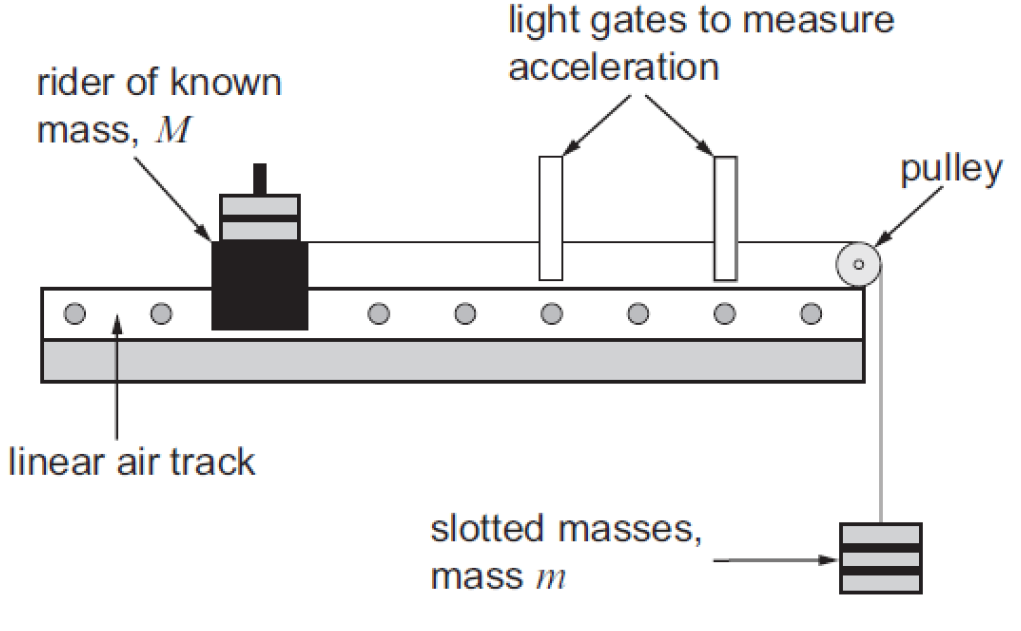
\includegraphics[width=\textwidth]{fma.PNG}
\caption{Newton's law experiment. Note that an air-track is not strictly necessary, we're trying to minimise the effect of friction on the system.}
\end{figure}
   
\subsection{Experimental Method:}  
Fix the thread to the rider and attach five slotted 5 gram masses to the other end as shown in the diagram. Set the light gates to record the acceleration and allow the slotted masses to fall to the ground. Record the gravitational force, mg and the acceleration, a. Remove one of the slotted masses and place it on the rider (so keeping the total mass of the system constant).   
Repeat the experiment until all the different accelerating masses have been removed. Plot a graph of acceleration (y-axis) against gravitational force, $mg$ (x-axis). This should be a straight line through the origin. \sidenote{By using a scales to measure the combined mass of the system $M+,m$ you could check that the gradient is equal to $1/(M+m)$}

%%%%%%%%%%%
%\newpage
\section{Determination of Young modulus of a metal in the form of a wire}

\subsection{Theory:}  $\text{Young modulus}  =\frac{\text{Stress}}{\text{Strain}}$  or $ E  =\frac{F/A}{x/l}$  rearranging $E =\frac{Fl}{xA}$ 
where: 
\begin{align}
       F &= \text{applied load} \\       A &= \text{area of cross-section of the wire} \\       x &= \text{extension}  \\      l &= \text{original length} \\ 
\end{align}
       
If a graph of applied load, F (y-axis) is drawn against extension, x (x-axis) the gradient is $\frac{F}{x}$ and so: \[E = \text{gradient} \times \frac{l}{A}\]     
The original length $l$ can be measured and the area of the wire found using $A= \pi r^{2}$ hence $E$ can be determined.  
\subsection{Apparatus:}   
  \begin{figure}
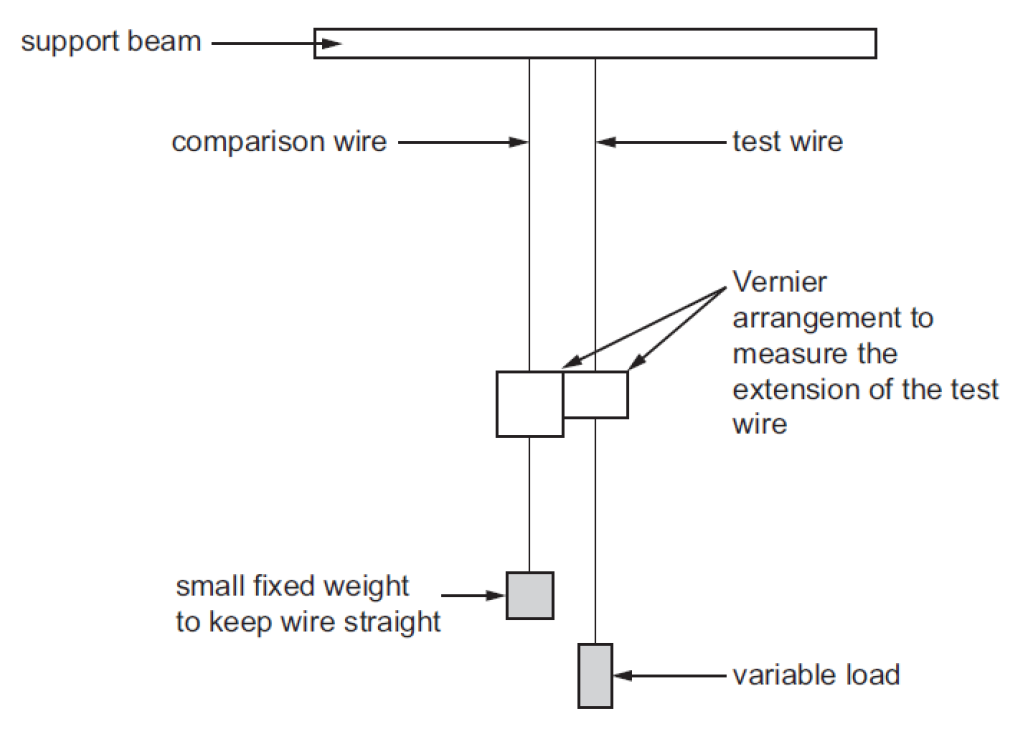
\includegraphics[width=\textwidth]{youngmod.PNG}
\caption{Young's Modulus apparatus}
\end{figure}
  
\subsection{Experimental Method:}  
Hang two identical wires from a beam and attach a scale to the first wire and a small weight to keep it straight.\sidenote{We use this method to eliminate any thermal extension/contraction} Also put a small weight on the second wire to straighten it and a Vernier scale linking with the scale on the comparison wire. Measure the original length, $l$, of the test wire and its diameter at various points along its length\sidenote{Measuring at several places along the length is a favourite of exam boards.}. Use this to calculate the mean cross sectional area $A$.  
Then place a load of \SI{5}{N} on the test wire and find the extension, $x$. Repeat this in $5$N steps up to at least $50$N. Plot a graph of load (y-axis) against extension (x-axis) and calculate the gradient. Use this to find a value for the Young modulus. 

%%%%%%%%%%%
%\newpage
\section{Investigation of the force-extension relationship for rubber}
\subsection{Theory:}  
Rubber is an example of a polymer with weak cross bonds. Natural rubber is a polymer of the molecule iso-prene. It has weak van der Waals cross-bonds and only a few covalent (strong) cross-bonds.   
\subsection{Apparatus:} 
\begin{itemize}
\item Rubber band of cross-section approximately 1 mm by 2 mm 
\item Clamp and stand G-clamp to secure (if required) 50 g mass holder plus a number of 50 g masses 
\item Optical pin (for use as a pointer if required) 
\item Metre rule (resolution $\pm 0.001$m) Micrometer (resolution $\pm 0.01$mm)
\end{itemize}
\begin{marginfigure}
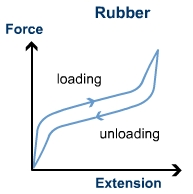
\includegraphics{hyst.jpg}
\caption{Hysteresis graph for rubber band}
\end{marginfigure}
\subsection{Experimental Method:}  
Hang a (cut) rubber band of (approximate) cross-section 1 mm by 2 mm vertically from a stand, boss and clamp. The base of the stand should be secured using a G-clamp. Hang a 50 gram mass holder from the band. Place a metre rule as close as possible to the mass holder. The length can be read using an optical pin attached to the base of the mass holder.
Measure the length, width and thickness of the rubber when it is supporting the 50 gram holder. Try to avoid squashing the rubber with the micrometer screw gauge. Increase the mass in 50 gram steps, measuring the extension each time. Continue until the band breaks.\sidenote{If, instead of testing to failure, you now unload the masses and measure the extension you can measure the elastic \emph{hysteresis} - the work done in rearranging the internal structure of the rubber.} Plot the force - extension curve and determine the Young modulus from the linear section.  
%%%%%%%%%%%
%\newpage
\section{I-V characteristics of the filament of a lamp and a metal wire at constant temperature}
\subsection{Theory:} 
Ohm's law states that for a conductor the current, I, is directly proportional to the potential difference, V, provided physical factors such as temperature and pressure remains constant.  Therefore by plotting the I-V characteristic of each of, a metal wire and a filament lamp, the validity of Ohm's law as applicable to each of these components can be determined. A graph of I against V is linear for a metal wire and non-linear for a filament of a lamp. 
\subsection{Apparatus:}
\begin {itemize}
\item Variable d.c. voltage supply 
\item Switch 
\item Ammeter 
\item Voltmeter 
\item Component either in the form of a filament bulb e.g. 12 V, 24 W bulb or a metal wire e.g. 1 m length of constantan mounted on a wooden batten 
\end{itemize}
\begin{marginfigure}
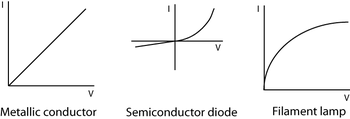
\includegraphics[]{vigraphs.png}
\caption{VI graphs of common components}
\end{marginfigure}

\subsection{Experimental method:} 
The circuit should be set up as in figure \ref{V-I}.
\begin{figure}
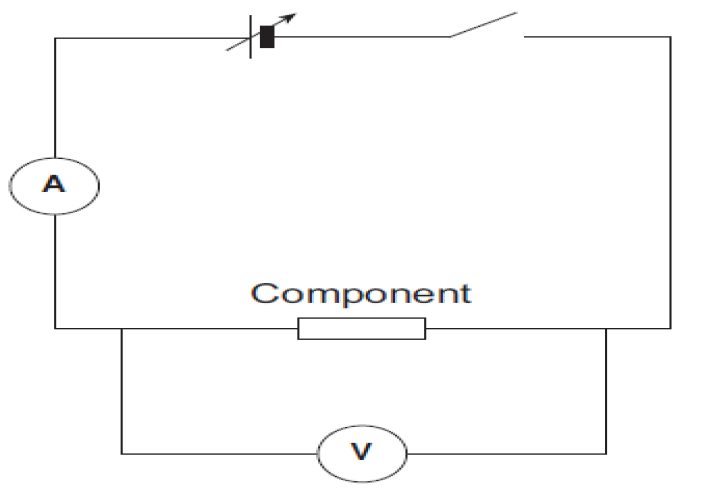
\includegraphics[width=\textwidth]{vicac.PNG}
\caption{V-I Characteristics set-up.\newline Note the variable powersupply and the switch. This basic circuit is used to investigate almost every electrical component}
\label{V-I}
\end{figure}

 
Starting with the output of the variable d.c. voltage supply set to its minimum value, slowly increase the value of the applied voltage. The current through the component and the potential difference across the component should be recorded for a range of values of the applied voltage. A graph of current against voltage should then be plotted. This procedure can be repeated for different components.
%%%%%%%%%%%
%\newpage
\section{Determination of the internal resistance of a cell}
\subsection{Theory:} 
\sidenote{I've tried to be quite clear here and give a bit of extra detail. Internal resistance is a favourite of examiners and I'd be amazed if this experiment didn't show up in some way}When charge flows through a cell it is given energy by the cell.
The number of joules of energy given to each coulomb of charge that passes through the cell is the e.m.f.\sidenote{e.m.f. is an abbreviation for electromotive force.} of the cell.
The energy can only be transferred to the charges at a finite rate, we model this as the cell having resistance. This model resistance is called the internal resistance of the cell. A cell can be thought of as a source of e.m.f. with a resistor connected in series.\begin{marginfigure}
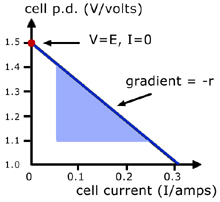
\includegraphics[]{intr.jpg}
\caption{Internal resistance graph}
\end{marginfigure}
When current flows through the cell a voltage develops across the internal resistance. This voltage is not available to the circuit so it is called the lost volts, ($V_{L}$).
$V_{L}$ can also be written as $Ir$
The voltage across the ends of the cell is called the terminal potential difference, ($V_{t.p.d}$).
$V_{t.p.d}$ can also be written as $IR$
Because voltage is a measure of energy, and energy is always conserved, the e.m.f. of a cell is equal to the sum of its terminal potential difference, ($V_{t.p.d}$), and the lost volts, ($V_{L}$).
This gives rise to the equation: \[E = V_{t.p.d.}+ V_{L}\]

This equation can be written in different forms, e.g. $E = I (R + r)$

The most common form of the equation used for determining the internal resistance is $V =E-Ir$ where $V$ is the terminal p.d. of a cell; $E$ is the emf of the cell; $I$  the current flowing in the circuit and $r$ is the internal resistance.  $V = IR$ and the equation can be re-written as $ R=\frac{E}{I}-r$.  Therefore a graph of $R$ against $1/I$  should be linear.   
\subsection{Apparatus:} 
\begin{itemize}
\item Cells - e.g. 3 or 4 1.5 V `D' type batteries connected in series
\item Switch 
\item Ammeter or multimeter set to A range - \SI{\pm 0.01}{A}
\item Various resistor values \SIrange{0}{60}{\Omega}
\end{itemize}
\subsection{Experimental method:} 
The circuit should be set-up as follows:  
\begin{figure}
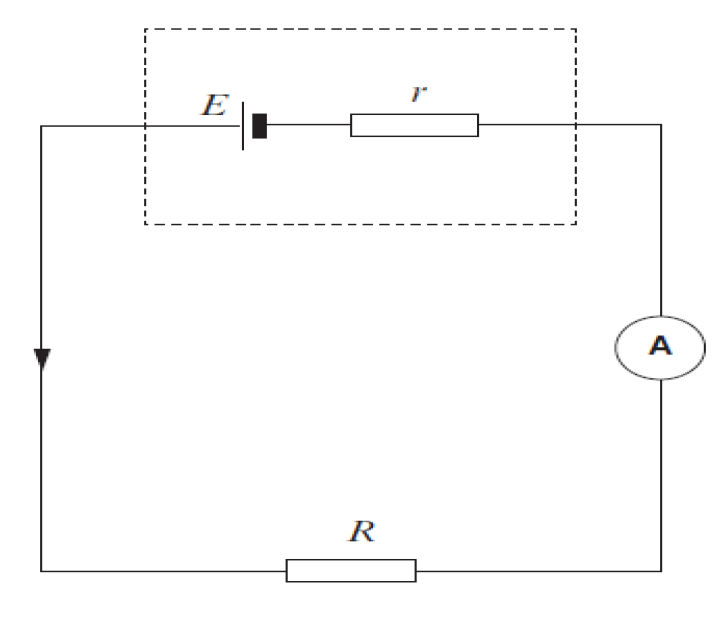
\includegraphics[width=\textwidth]{internalres.PNG}
\end{figure}

The resistor values should be varied and the current values recorded. Plot a graph of $R$  (y-axis) against $1/I$  (x-axis).  The graph should be a straight line with the intercept on the y-axis which is equal to the value of the internal resistance. 
%%%%%%%%%%%
%\newpage
\section{Measurement of the intensity variations for polarisation}
\subsection{Theory:} 
The light waves in a ray of light from a lamp have vibrations in all planes and directions.  The light is unpolarised.  When the light passes through a polaroid filter; the vibrations will be in one plane or direction only.  In the experiment with two pieces of polaroid, the first polarises the light.  The light will then not pass through the second polaroid if the direction in which the second filters polarises light is at right angles to the polarising direction of the first polaroid.
\subsection{Apparatus:} \begin{itemize} 
\item Two pieces of polaroid 
\item Lamp e.g. 24 W, 12 V bulb in holder  
\end{itemize}
\subsection{Experimental method:} 
Investigate the variation in intensity by looking through the lamp through both polaroids and rotating one of the polaroids through \SI{360}{\degree}.
\begin{figure}
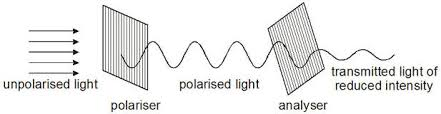
\includegraphics[width=\textwidth]{malus.jpg}
\caption{Investigating the Polarisation of light. When the full version (not on the spec) is done, the intensity of light and the angle of the analyser relative to the polariser is measured. The experiment is used to test malus's law. According to malus, when completely plane polarized light is incident on the analyzer, the intensity of the light transmitted by the analyzer is directly proportional to the square of the cosine of angle between the transmission axes of the analyzer and the polarizer.}
\end{figure} 
Note the change in intensity that occurs. 
%%%%%%%%%%%
%\newpage
\section{Determination of wavelength using Young's double slits}
\subsection{Theory:} Young's interference experiment, also called Young's double-slit interferometer, was the original version of the modern double-slit experiment, performed at the beginning of the nineteenth century by Thomas Young. This experiment played a major role in the general acceptance of the wave theory of light. The fringe spacing, $\Delta y $ is given by the equation$\Delta y = \frac{\lambda D}{d}$ where $\lambda$ is the wavelength of the light; $D$ is the distance from the slits to the screen where the fringes are viewed and $d$ is the distance between the slits.  A graph of $\Delta y$ against $D$ should be a straight line and the gradient can be used to determine the wavelength of the light. 
\subsection{Apparatus:}
\begin{itemize}
\item Laser pen 
\item Stand and clamp 
\item Double slit 
\item Screen 
\item Metre rule 
\item 30 cm ruler or digital callipers
\end{itemize}
\subsection{Experimental method:} 
The apparatus should be set-up as follows:   
\begin{figure}
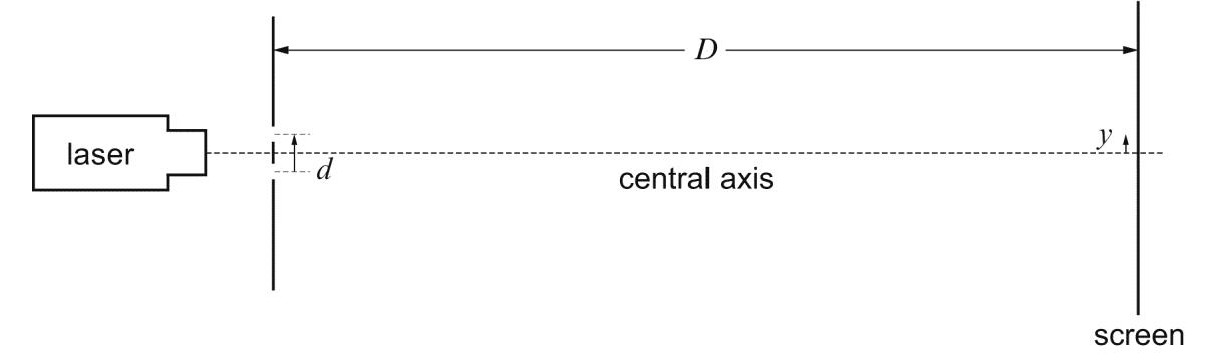
\includegraphics[width=\textwidth]{youngs.PNG}
\caption{Young's Slits experiment}
\end{figure}

Measure the fringe spacing
\begin{marginfigure}
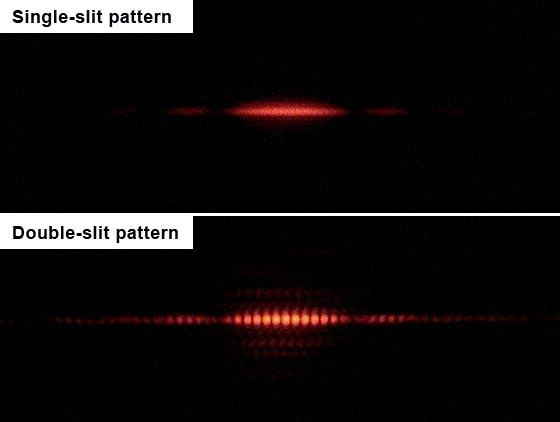
\includegraphics[]{singledouble.jpg}
\caption{Fringe pattern for red light of \SI{633}{nm}.}
\end{marginfigure} $\Delta y$, the spacing between the slits, $d$, and the distance, $D$, from the slits to the screen using either the ruler or digital callipers.  Vary the distance, $D$ in equal intervals. Plot a graph of the fringe spacing $\Delta y$ (y-axis) against the slit-screen distance $D$  (x-axis). This should be a straight line through the origin.  
If the fringes are close together; $\Delta y$ can be determined by measuring the separation of a number of fringes. So determine by dividing the distance by the number of fringes measured.   
%%%%%%%%%%%
%\newpage
\section{Determination of wavelength using a diffraction grating}
\subsection{Theory:} 
The diffraction grating equation is given by $n \lambda  =d\sin \theta$. The spacing between the lines in a diffraction grating is usually specified or can be found from the grating ruling.
\begin{marginfigure}
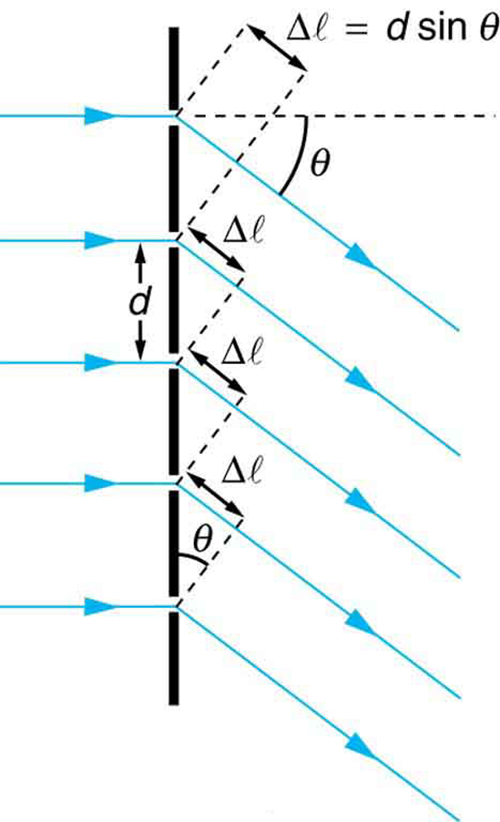
\includegraphics[]{diffraction.jpg}
\caption{Geometry of diffraction}
\end{marginfigure} 
By measuring the angle $\theta$, the wavelength of the light can be determined. 
\subsection{Apparatus:}
\begin{itemize}
\item Laser 
\item Diffraction grating of known $d$ value or ruling e.g. 300 lines \si{cm^-1} 
\item Metre rule 
\item Screen 
\item Stand and clamp for laser and grating 
\end{itemize}

\subsection{Experimental method:} 
The apparatus should be set-up as follows:  
\begin{figure}
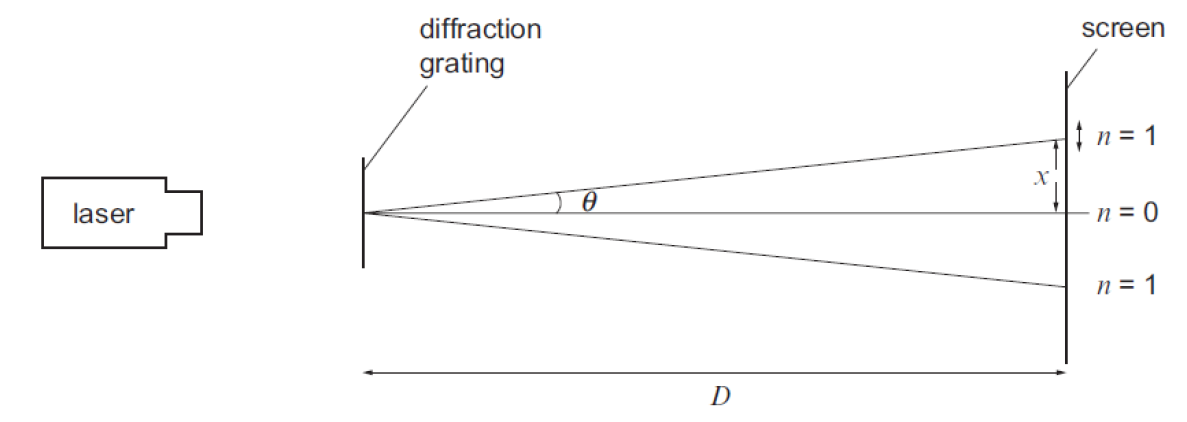
\includegraphics[width=\textwidth]{diffractiongrating.PNG}
\caption{Diffraction grating setup}
\end{figure}
The value of $\theta$ can be determined from $\tan \theta = \frac{x}{D}$. \\ 
Using the equation $n \lambda  =d\sin \theta$ then the wavelength can be determined for various orders of diffraction. 
%%%%%%%%%%%
%\newpage
\section{Determination of the speed of sound using stationary waves}
\subsection{Theory:} 
When resonance first occurs the length of air in the tube, $l$, plus a small end correction, $e$ (to account for the position of the tuning fork above the tube) will be equal to a quarter of a wavelength. Hence: 
\[l + e = \lambda/4 \] but \[ \lambda = c/f \] so   \[l = \frac{c}{4f}-e\] If a graph is plotted of $l$ (y-axis) against $1/f$ (x-axis) it should be a straight line with a small negative y-intercept. \begin{marginfigure}
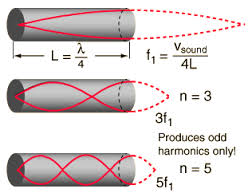
\includegraphics[]{waves.jpg}
\caption{Standing waves in an open ended pipe}
\end{marginfigure}
The gradient of the graph equals $c/4$, and so the speed of sound, $c$, can be found. The small negative intercept will give the end correction. 
\subsection{Apparatus:}   
\begin{figure}
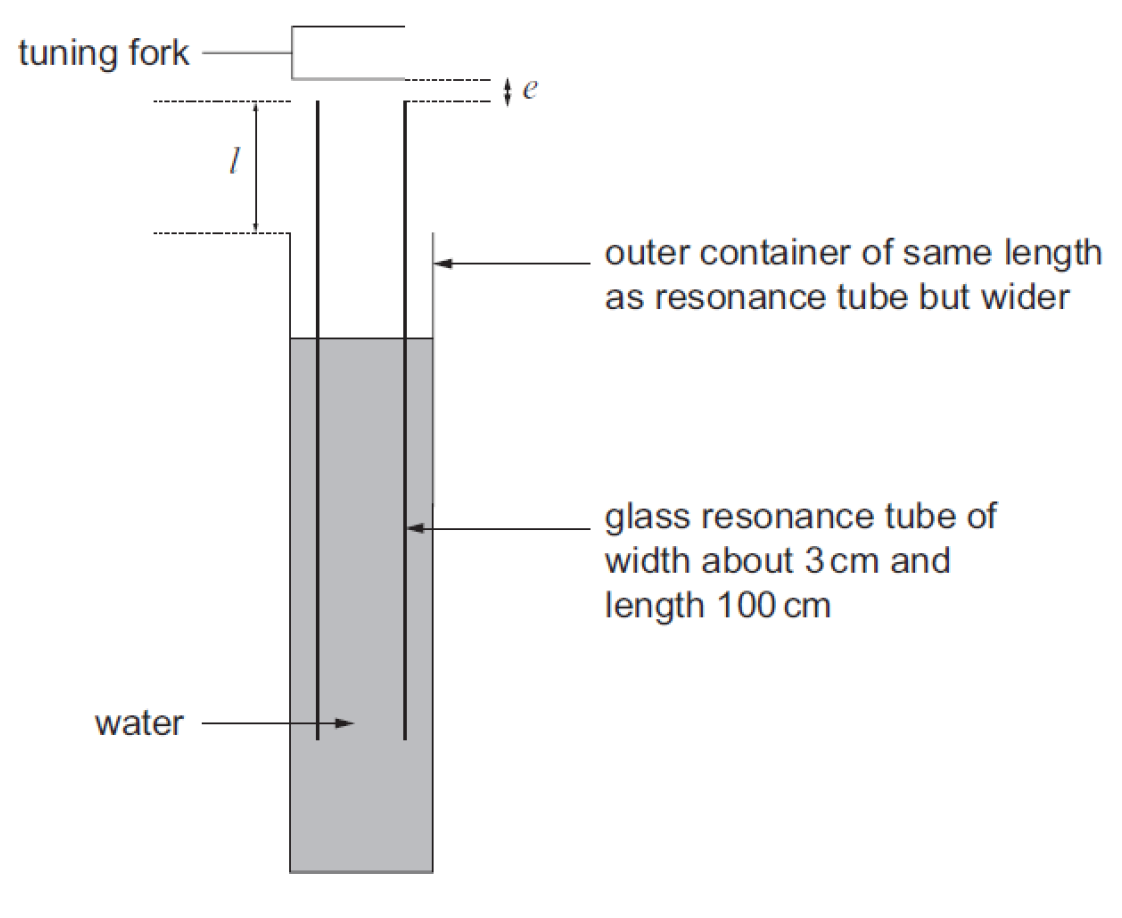
\includegraphics[width=\textwidth]{speedsound.PNG}
\end{figure}
   
A range of at least five different tuning forks will be needed along with a metre ruler of resolution \SI{\pm0.001}{m}. 
\subsection{Experimental method:}

Initially place the resonance tube as deep as possible into the water. Then gradually raise it. As this is being done hold a vibrating tuning fork over the top. When resonance occurs (a loud sound will be heard) measure the length of the tube above the water level.  Repeat the above for each of the tuning forks. Plot a graph of length (y-axis) against 1/frequency (x-axis). Use the gradient to determine a value for the speed of sound.
%%%%%%%%%%%
%\newpage
\section{Determination of resistivity of a metal}
\sidenote{There are lots of possible experiments here. So long as you are systematic in changing only one variable in $R=\frac{\rho l}{A}$}
\subsection{Theory:}  Resistivity, $\rho$ can be found using the equation $R=\frac{\rho l}{A}$ where $l$ is the length of the wire, $A$ the cross-sectional area and $R$ the resistance.\begin{marginfigure}
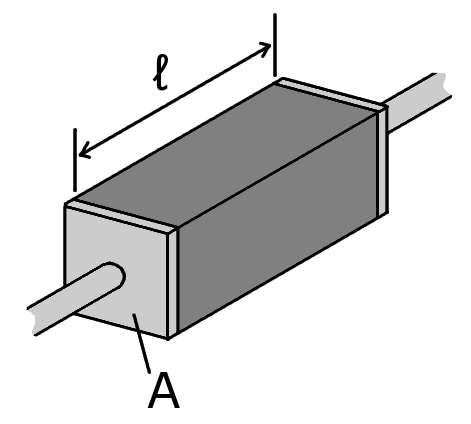
\includegraphics[]{resistivity.png}
\caption{Geometry of resistivity}
\end{marginfigure} This can be compared with the equation for a straight-line $ y = mx +c$. A graph plotted of $R$ (y-axis) against $l$ (x-axis) will be a straight line through the origin of gradient $\frac{\rho}{A}$. The cross sectional area can be found using $A=\pi r^{2}$ and the resistivity calculated by $ \rho = \text{gradient} \times A$.  
\subsection{Apparatus:} 
\begin{figure}
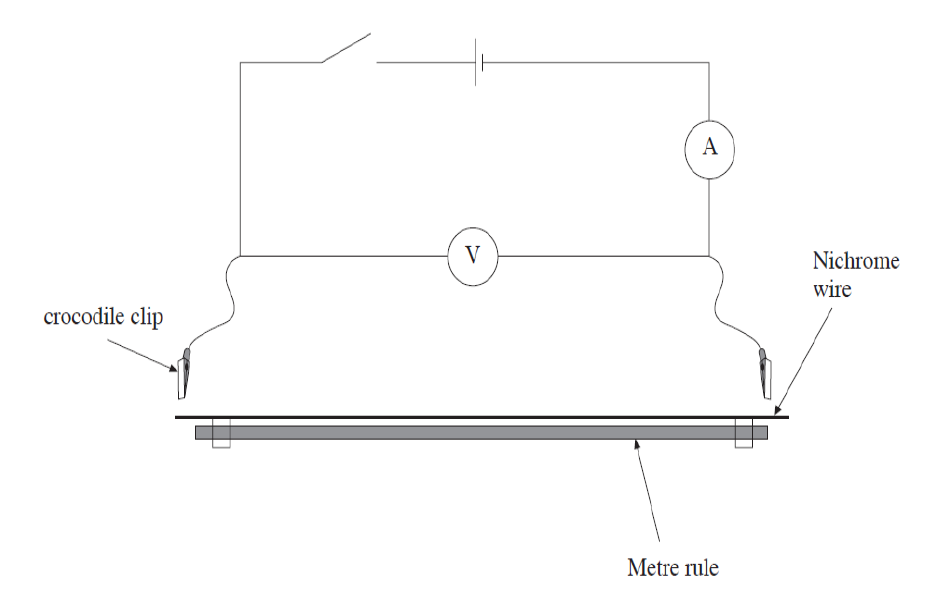
\includegraphics[width=\textwidth]{resist.PNG}
\caption{Experimental set-up for Resistivity of a wire investigation}
\end{figure}
\begin{itemize}
\item leads 
\item ammeter 
\item voltmeter 
\item 1.5 V `D' type battery 
\item metre rule 
\item 110 cm length of nichrome wire
\item 1  micrometer / vernier callipers (resolution \SI{\pm 0.01}{mm})  
\item 30 cm ruler (resolution \SI{\pm 0.001}{m})  
\end{itemize}
\subsection{Experimental Method:}  
Leaving one crocodile clip fixed at one end of the wire, the other clip should be moved along at suitable intervals e.g. every 10 cm / 20 cm to cover the whole range of the wire. Readings on the voltmeter and ammeter should be noted for each length and the resistance determined using $R = \frac{V}{I}$ . The diameter of the wire can be found using a micrometer or Vernier callipers and the cross-sectional area determined. Plot a graph of $R$ (y-axis) against $l$ (x-axis) and calculate the resistivity using:  $\rho = \text{gradient} \times A$. 
%%%%%%%%%%%
%\newpage
\section{Investigation of the variation of resistance with temperature for a metal wire}
\subsection{Theory:} 
Resistance increases with temperature for metals in a linear relationship. This practical will enable data to be obtained to investigate this relationship. \sidenote{A common substitution is to swap the wire in the investigation for a thermistor. Thermistors are semiconductor devices that have the reversed behaviour to normal wires. As their temperature increases, the resistance of a thermistor \emph{decreases}}.
\subsection{Apparatus:}
\begin{itemize}
\item Bunsen burner; tripod, gauze and stand 
\item 250 ml beaker of water 
\item Ice \marginnote{Because the effect of resistance change with temperature is small, it is important to cover as large a range of temperatures as is safe and practical. In an A-level lab it would be possible to get down to about \SI{-40}{\degree C} and up to about \SI{1200}{\degree C}. These extreme temperatures are dangerous however and would need particular precautions}
\item Thermometer \SIrange{0}{100}{\degree C} 
\item Multimeter set on ohm range to measure resistance 
\item Copper coil 
\item Stirrer
\end{itemize}

\subsection{Experimental method:}
The circuit should be set up as follows:  
\begin{figure}
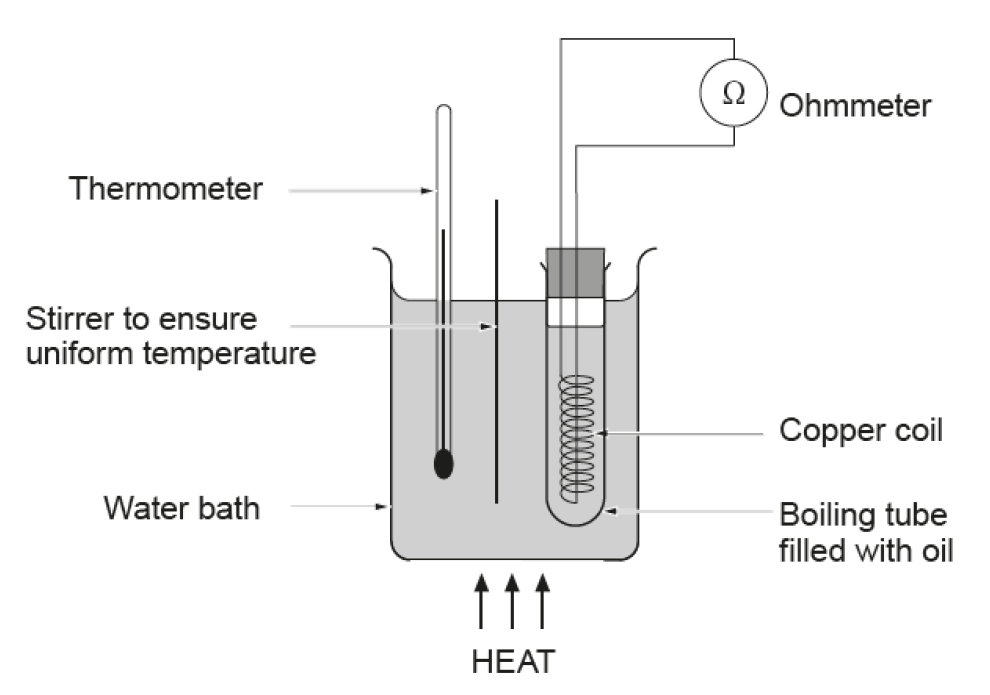
\includegraphics[width=\textwidth]{restemp.PNG}
\caption{Resistance of a wire with Temperature}
\end{figure}
The water bath should be heated and the water stirred continuously in order to ensure an even temperature throughout the water bath.  Once the required temperature has been reached then remove the heat and record the reading of resistance or take the ammeter and voltmeter readings. This process should be repeated at intervals until the water boils.  
Repeat the experiment during cooling. Plot a graph of resistance (y-axis) against temperature (x-axis). This should be a straight line through the origin.  
An ice water mixture can be used to record the resistance at a temperature of \SI{0}{\degree C}. 
%%%%%%%%%%%
%\newpage
\section{Measurement of the refractive index of a material}
 \subsection{Theory:}  
The refractive index, $n$, of a material can be determined from the equation $\sin \theta_{i} = \sin \theta_{r}$ where $n$ = refractive index, $\theta_{i}$is the angle of incidence and $\theta_{r}$ is the angle of refraction. \begin{marginfigure}
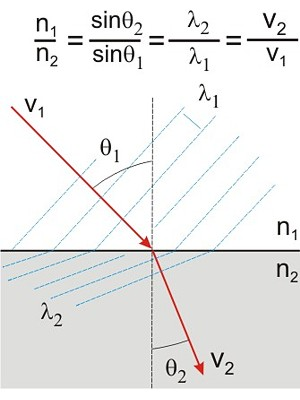
\includegraphics[]{refrac.jpg}
\caption{Refractive index measurement}
\end{marginfigure} The above equation assumes that the incident ray is travelling in air.  A graph of $\sin\theta_{i}$ (y-axis) against $\sin \theta_{r}$ (x-axis) will give a straight line through the origin and the gradient is equal to the refractive index, $n$.  
\subsection{Apparatus:} 
\begin{itemize}
\item Suitable white light source e.g. ray box fitted with a single slit to produce a narrow parallel beam of light 
\item Power supply for ray box and connecting leads 
\item Rectangular block of glass or Perspex 
\item 1 or 2 sheets of plain paper 
\item Protractor 
\item 30 cm ruler
\end{itemize}
\subsection{Experimental Method:}  
The following arrangement should be set-up.  
\begin{figure}
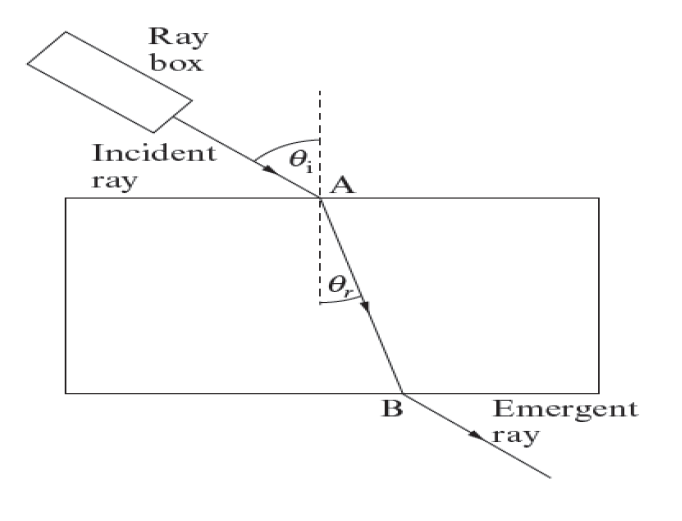
\includegraphics[width=\textwidth]{snells.PNG}
\end{figure}
The angle of refraction $\theta_{r}$ can be measured by drawing in the line joining the incident and emergent rays for different values of the angle of incidence\sidenote{Particular care should be taken here. The more precise the drawing, the better the final results.}. The angles can be measured using the protractor after drawing in the normals\sidenote{the ``normal'' is a line at \SI{90}{\degree} to a surface. In this case it is at \SI{90}{\degree} to the glass block, as shown by a dotted line in the diagram}. A graph of $\sin\theta_{i}$ (y-axis) against$\sin \theta_{r}$(xaxis) can be plotted which should give a straight line. A value of $n$ can then be determined from the gradient. 
%%%%%%%%%%%
%\newpage
\section{Determination of h using LEDs}
\subsection{Theory:} The Planck constant, $h$, can be determined by using a light emitting diode (LED) and measuring the minimum voltage, $V_{min}$, at which light is just emitted by the diode. \sidenote{The energy levels in the LED are quantised, and they are constructed such that their emissions are monochromatic. Because energy is conserved, the only light that the LED can emit will have an energy corresponding to the energy level transition inside the material. \newline Potential difference is a measure of the energy difference between two points. The potential required to light the LED must therefore be the energy of the photons released. Photon energy is given by $E=hf$, where $h$ is planck's constant and $f$ is the frequency of light.} The Planck constant can then be determined from the equation $V_{min}=\frac{hc}{e\lambda}$  where $c$ is the speed of light \SI{3.00e8}{ms^-1} and $e$ is the electronic charge, \SI{1.60e-19}{C}.  A graph of $V_{min}$ against $1/\lambda$ should be a straight line with the gradient equal to $V_{min}=\frac{hc}{e}$. \sidenote{Many experiments have equations in the form $y=mx+c$. You should expect to have to match the variables in an equation with the parts of an equation of a straight line. It would be unsurprising to have a question requiring you to calculate gradients and Y-intercepts}

\subsection{Apparatus:} \begin{itemize}
\item Variable d.c. power supply 
\item \SI{1}{k \Omega} protective resistor 
\item Voltmeter (resolution \SI{\pm0.01}{V}) [multimeter set to appropriate range] \item Connecting leads 
\item Various LEDs - with known wavelengths
\end{itemize}
\subsection{Experimental Method:} The circuit should be set-up as follows: 
\begin{figure}
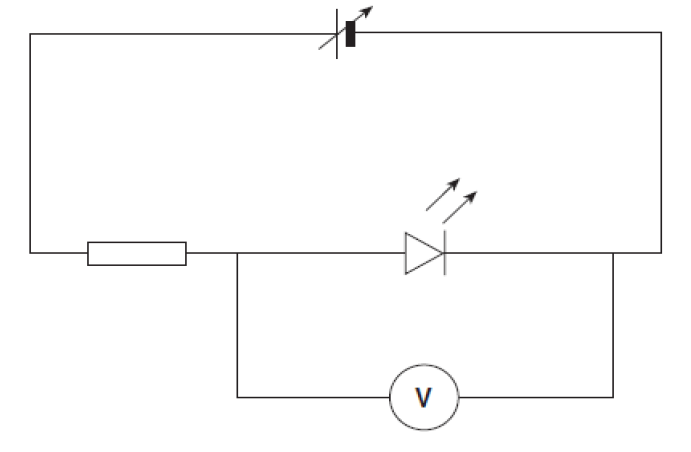
\includegraphics[width=\textwidth]{plank.PNG}
\end{figure}

The voltage should be varied until light is just emitted by the LED. Record the voltage it corresponds to $V_{min}$. The LED should be replaced and the procedure repeated for LEDs with different wavelengths of light.  Plot a graph of $V_{min}$ (x-axis) against $1/ \lambda$  (y-axis) and use it to determine a value for $h$. 
\end{document}